\section{Diagrama de Fazes}

Def: O diagrama de fases de um dado sistema indica que tipo de microestrutura estará presente, em uma determinada temperatura e composição. É um diagrama termodinâmicos, que não indica a velocidade das reações.

A solubilidade é um dos fatores que interferem diretamente na formação de uma ou mais fases. Pois, quando o sistema ultrapassar o limite de solubilidade uma segunda fase será formada.

Uma liga metálica policristalina pode apresentar mais de um fase.

A figura abaixo mostra como a solubilidade uma determinada substância em relação a outra pode alterar em função da temperatura.


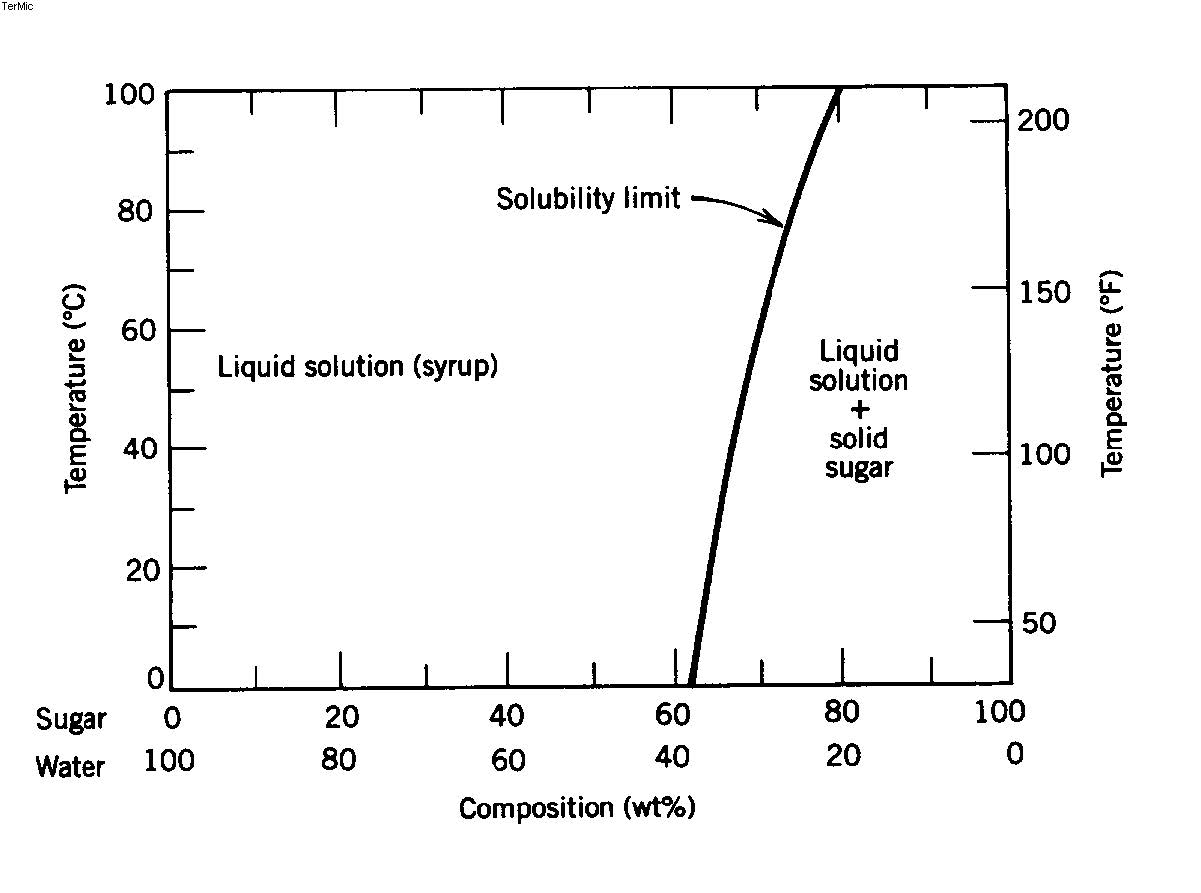
\includegraphics[scale=0.3,trim={0 0 0 0}]{figures/soluTemp}

Diagrama de fases de substância pura: 

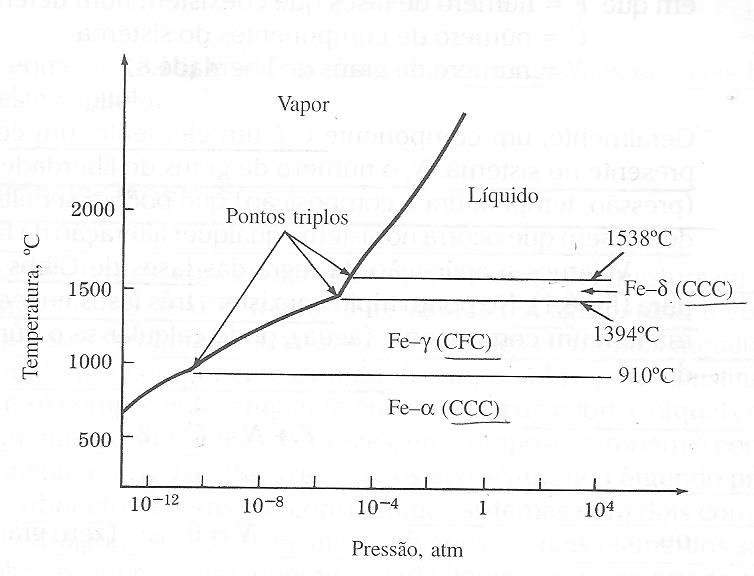
\includegraphics[scale=0.4,trim={0 0 0 0}]{figures/diagramFe}

A partir do DIAGRAMA DE FASES, para um dado \emph{teor de soluto} e uma dada \emph{temperatura} podemos predizes:


\begin{itemize}
	\item que fases são \emph{termodinamicamente} estáveis.
	\item a composição de cada uma delas
	\item a quantidade de cada uma delas
\end{itemize}


\section{Solubilidade entre Componentes}

{\normalsize Sistema Binário Isomorfo: com solubilidade total no líquido e no sólido.}




Sistema Binário Isomorfo:

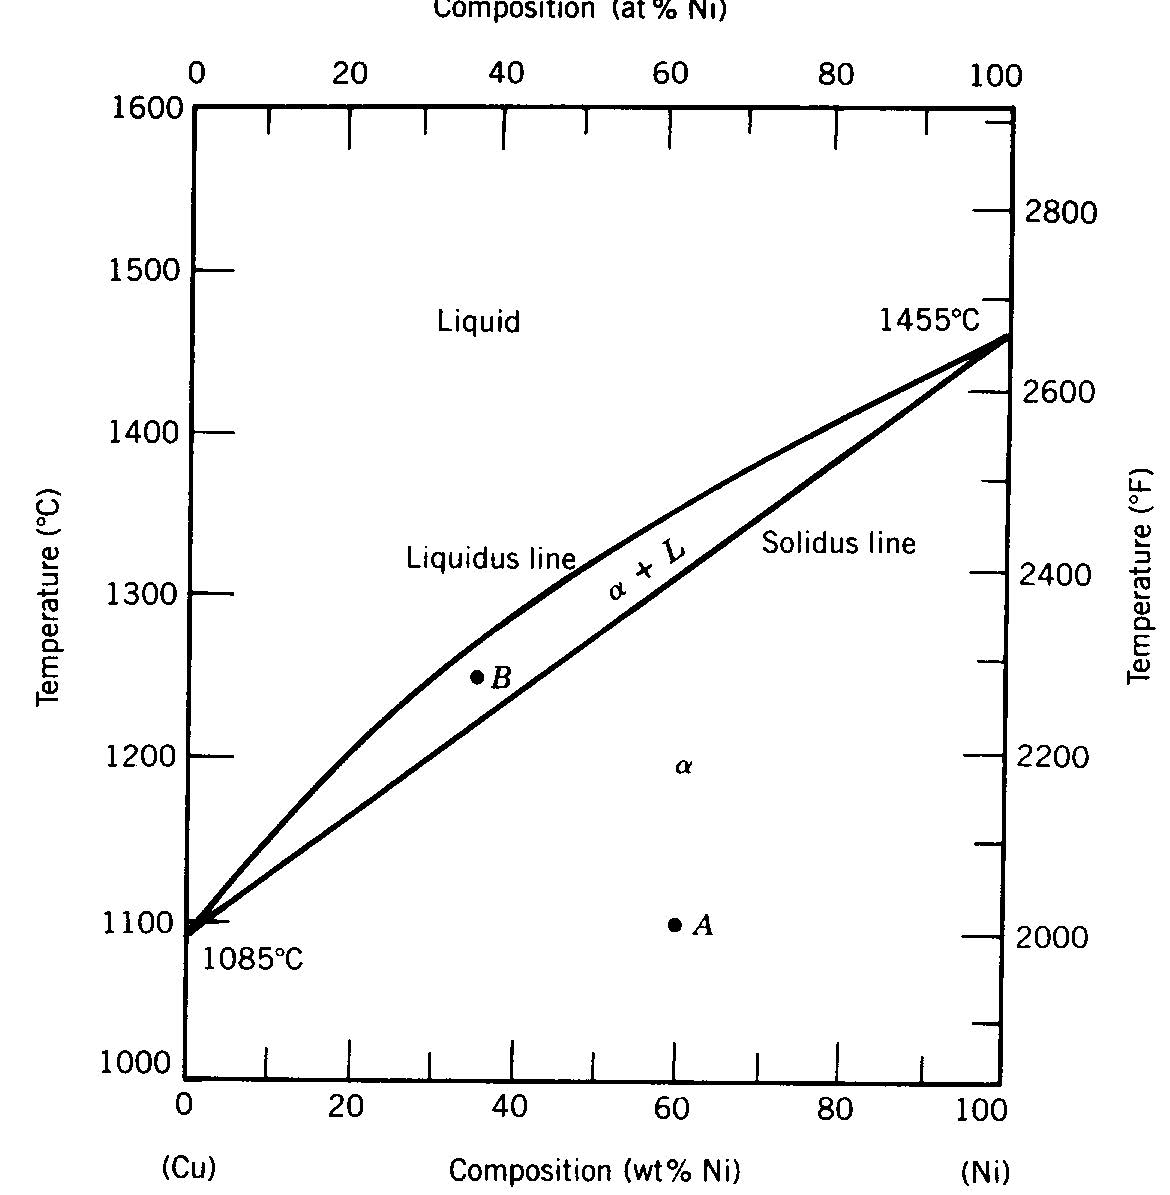
\includegraphics[scale=0.4,trim={0 0 0 0}]{figures/binIso}

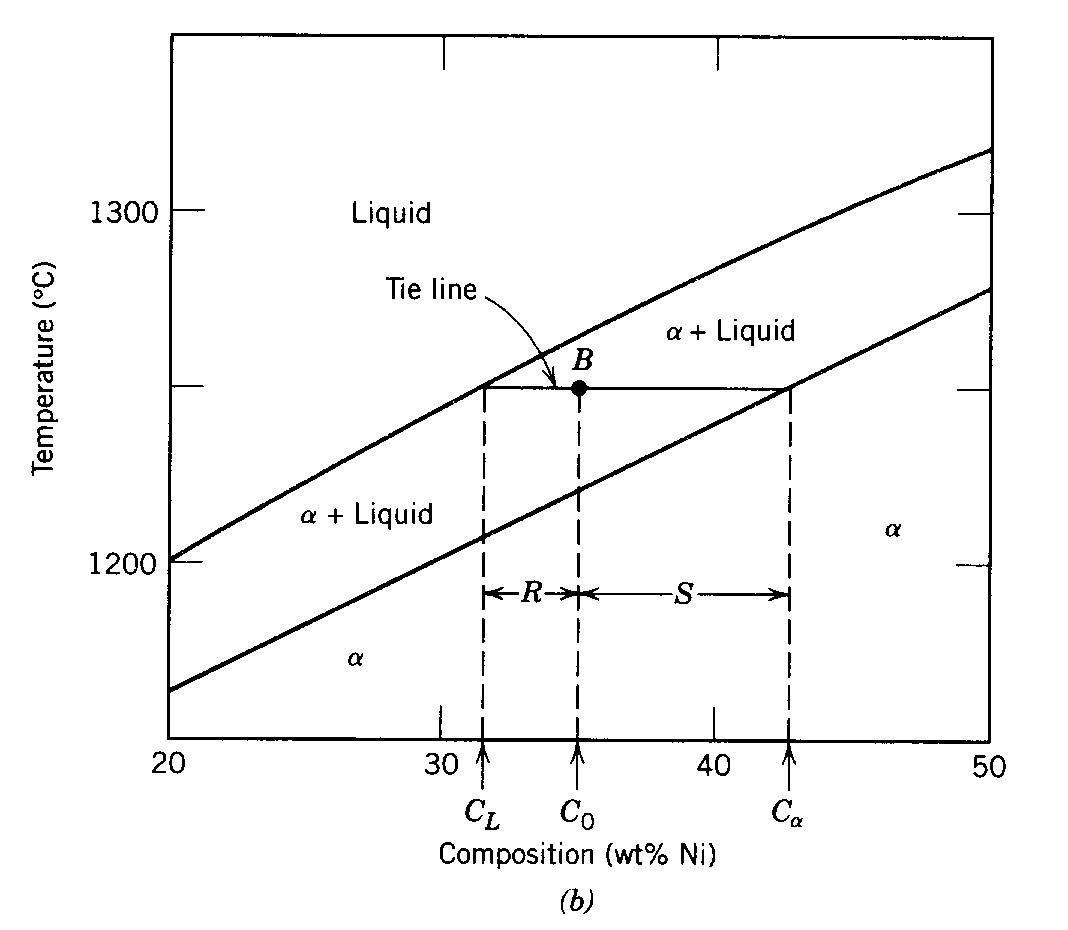
\includegraphics[scale=0.4,trim={0 0 0 0}]{figures/binIso2}

\begin{equation}\label{key}
\mathrm{C}_{0}=\mathrm{C}_{\mathrm{L}} \mathrm{W}_{\mathrm{L}}+\mathrm{C}_{\mathrm{S}} \mathrm{W}_{\mathrm{S}}
\end{equation}

\begin{equation}\label{key}
\mathrm{W}_{\mathrm{L}}+\mathrm{W}_{\mathrm{S}}=1
\end{equation}

\begin{equation}\label{key}
\mathrm{W}_{\mathrm{S}}=\frac{\left(\mathrm{C}_{0}-\mathrm{C}_{\mathrm{L}}\right) }{\left(\mathrm{C}_{\mathrm{S}}-\mathrm{C}_{\mathrm{L}}\right)}
\end{equation}

\begin{equation}\label{key}
W_{L}=\frac{\left(C_{S}-C_{0}\right) }{\left(C_{S}-C_{L}\right)}
\end{equation}

No diagrama:

\begin{itemize}
	\item Fração mássica da fase líquida: $W_{L}$= S / R + S
	\item Fração mássica da fase sólida $W_{S}$= R / R + S
\end{itemize}



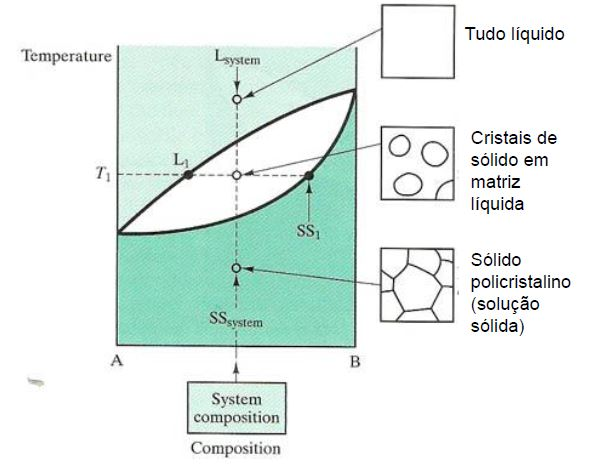
\includegraphics[scale=0.4,trim={0 0 0 0}]{figures/fases}

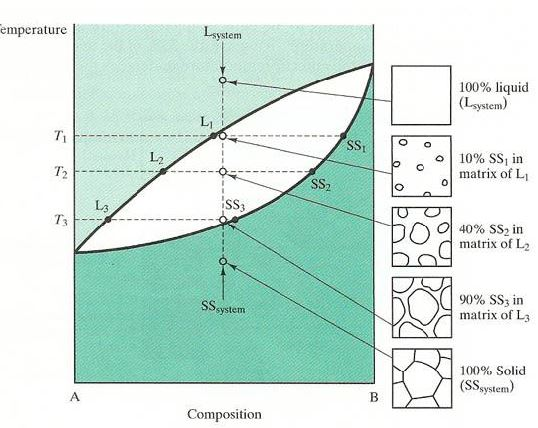
\includegraphics[scale=0.4,trim={0 0 0 0}]{figures/fases2}

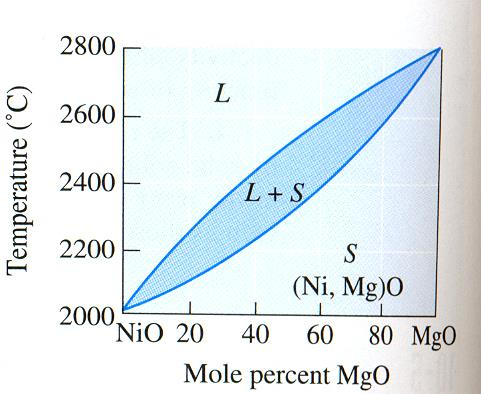
\includegraphics[scale=0.4,trim={0 0 0 0}]{figures/subsCompos}

A medida que a liga resfria, a solidificação avança e a composição das fases é alterada.




{\normalsize  Sistema Binário sem qualquer solubilidade: sem formação de solução solida.}

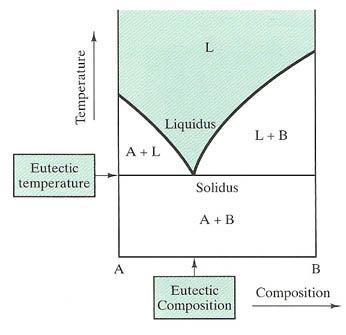
\includegraphics[scale=0.4,trim={0 0 0 0}]{figures/semQ}

Microestrutura:

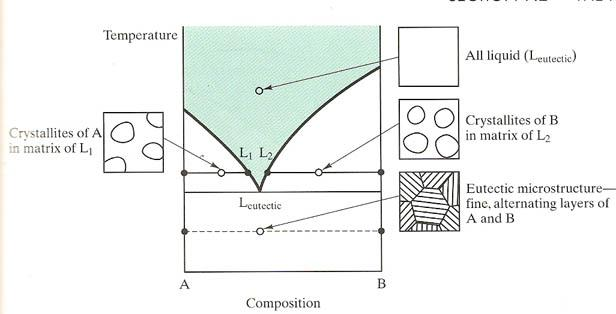
\includegraphics[scale=0.4,trim={0 0 0 0}]{figures/microSemQ}


{\normalsize Sistema Binário com solubilidade parcial: com reação eutética e/ou eutetóide.}

Com reação eutética:

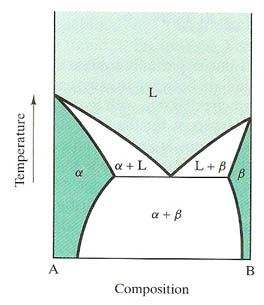
\includegraphics[scale=0.4,trim={0 0 0 0}]{figures/eute}

\begin{equation}\label{key}
L \leftrightarrow S_{1} = S_{2}
\end{equation}

Micro estrutura:

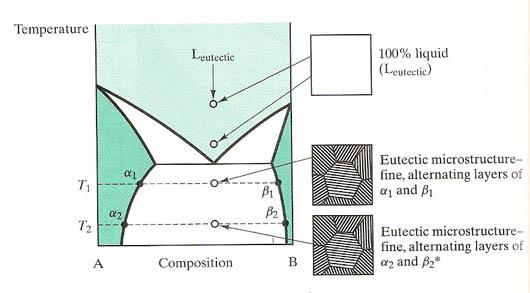
\includegraphics[scale=0.4,trim={0 0 0 0}]{figures/microEute}

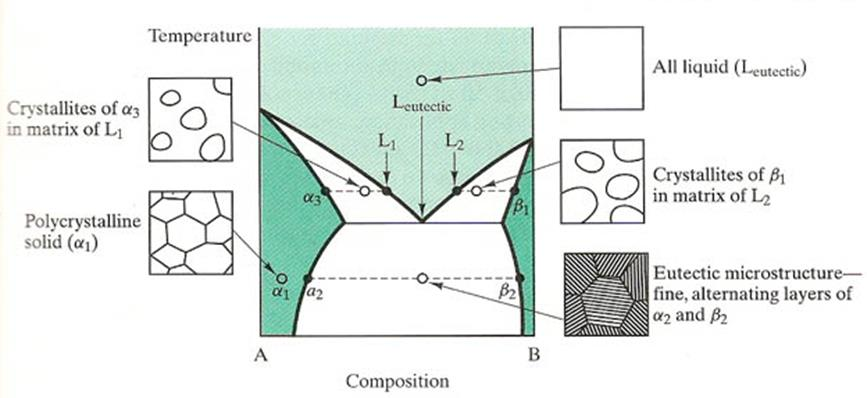
\includegraphics[scale=0.4,trim={0 0 0 0}]{figures/microEute2}



